\documentclass[12pt]{article}
\usepackage{sbc-template}
\usepackage[T1]{fontenc}
\usepackage[utf8]{inputenc}
\usepackage[brazil]{babel}
\usepackage{graphicx,url,booktabs,listings,xcolor}
\lstset{basicstyle=\ttfamily\footnotesize,frame=single,breaklines=true,columns=fullflexible,
  keywordstyle=\bfseries,morekeywords={MATCH,WHERE,WITH,RETURN,DISTINCT,LIMIT,IN,AS}}
\renewcommand{\lstlistingname}{Listagem}
\sloppy

\title{GraphRAG sobre Jogos Online: Recuperação Híbrida em Grafo de Conhecimento com Mitigação de Alucinações}
\author{Biel Aguiar, Thiago Rocha}
\address{Unipê Cruzeiro do Sul -- Ciência da Computação -- João Pessoa -- PB -- Brasil}
\begin{document}
\maketitle
\begin{abstract}
Retrieval-Augmented Generation (RAG) grounds language models in external text, but vector-only retrieval struggles with questions whose answer is spread across several documents and offers no way to say ``this is not in the base''. We present a GraphRAG/KAG system over online games built from 65 English Wikipedia articles. A Text-to-Graph pipeline extracts typed entities and relations with literal evidence, resolves 811 mentions into 351 canonical entities and loads a Labeled Property Graph into Neo4j with uniqueness constraints, range, fulltext and vector indexes, PageRank and Louvain. Retrieval fuses vector, fulltext and dictionary entity linking, multi-hop traversal, all-shortest-paths between anchors and an intent-directed query; generation is constrained to cited triples and checked by a citation verifier. On 21 in-domain questions and 5 out-of-domain ones, the graph context reached 100\% full support against 71.4\% for a vector baseline (2+ hops: 100\% vs. 76.9\% recall) and refused all out-of-domain questions, which the baseline cannot do.

\end{abstract}
\begin{resumo}
A Geração Aumentada por Recuperação (RAG) ancora modelos de linguagem em textos externos, mas a busca puramente vetorial falha em perguntas cuja resposta está espalhada em vários documentos e não oferece meios de dizer ``isso não está na base''. Este trabalho apresenta um sistema GraphRAG/KAG sobre jogos online construído a partir de 65 artigos da Wikipedia em inglês. Um pipeline Text-to-Graph extrai entidades e relações tipadas com evidência literal, resolve 811 menções em 351 entidades canônicas e carrega um grafo de propriedades rotulado (LPG) no Neo4j com restrições de unicidade, índices range, fulltext e vetoriais, PageRank e Louvain. A recuperação combina ligação de entidades vetorial, textual e por dicionário, travessia multi-hop, todos os caminhos mínimos entre âncoras e uma consulta dirigida pela intenção da pergunta; a geração é restrita a triplas citadas e conferida por um verificador de citações. Em 21 perguntas do domínio e 5 fora dele, o contexto do grafo teve suporte completo em 100\% das perguntas contra 71,4\% de um baseline vetorial (2+ saltos: recall de 100\% contra 76,9\%) e recusou todas as perguntas fora do domínio, o que o baseline não faz.

\end{resumo}
\section{Introdução}
Modelos de linguagem de grande porte (LLMs) respondem com fluência, mas produzem afirmações sem respaldo, as chamadas alucinações \cite{ji2023survey}. A Geração Aumentada por Recuperação (RAG) reduz o problema ao inserir no prompt trechos recuperados de uma base externa \cite{lewis2020rag}. Na forma mais comum, os documentos são divididos em trechos, cada trecho vira um vetor e a pergunta recupera os trechos mais próximos. Essa abordagem funciona bem quando a resposta está em um único trecho, mas tem dois limites conhecidos. O primeiro aparece em perguntas de vários saltos, em que cada fato está em um documento diferente: os trechos intermediários quase nunca são os mais parecidos com a pergunta. O segundo é a ausência de um critério para recusar: a busca vetorial sempre devolve os $k$ vizinhos mais próximos, mesmo quando nenhum deles tem relação com a pergunta.

GraphRAG e KAG (Knowledge Augmented Generation) atacam esses limites estruturando o conhecimento como um grafo antes da consulta \cite{edge2024graphrag,liang2024kag,peng2024survey}. Entidades e relações explícitas permitem seguir caminhos entre documentos, e a correspondência exata com nós do grafo dá um sinal objetivo de que a pergunta toca a base.

Este artigo descreve um sistema completo de perguntas e respostas sobre jogos online (MOBAs, battle royale, tiro, MMOs, sandbox, jogos mobile e campeonatos de e-sports). As contribuições são:

\begin{enumerate}\item um pipeline Text-to-Graph com extração tipada, descarte de relações sem evidência literal e resolução de entidades com travas lexicais;
\item uma modelagem LPG no Neo4j com restrições, índices range, fulltext e vetoriais, e propriedades calculadas por PageRank e Louvain;
\item uma recuperação híbrida que combina ligação de entidades por três canais, travessia multi-hop, caminhos mínimos e uma consulta dirigida pela intenção, com geração de Cypher por LLM sob trava de somente leitura;
\item uma interface que mostra o subgrafo usado, as consultas Cypher, os nós consultados e o nível de confiança;
\item uma avaliação contra RAG vetorial puro, com perguntas de um e de vários saltos e perguntas fora do domínio.
\end{enumerate}
O restante do texto está organizado assim: a Seção 2 apresenta a fundamentação; a Seção 3 descreve a arquitetura e cada etapa; a Seção 4 traz a avaliação; a Seção 5 discute limitações e a Seção 6 conclui.

\section{Fundamentação e trabalhos relacionados}
\textbf{Grafos de conhecimento e LPG.} Um grafo de conhecimento representa entidades como nós e fatos como arestas tipadas \cite{hogan2021kg}. No modelo de grafo de propriedades rotulado (LPG), nós e arestas têm rótulos e pares chave-valor, o que permite guardar, na própria aresta, a frase de origem e o documento de onde o fato veio. O Neo4j implementa esse modelo e a linguagem declarativa Cypher \cite{francis2018cypher,robinson2015graph}.

\textbf{RAG e GraphRAG.} O RAG original combina um recuperador denso e um gerador \cite{lewis2020rag}. O GraphRAG da Microsoft constrói um grafo de entidades, detecta comunidades e resume cada uma para responder perguntas globais \cite{edge2024graphrag}. O HippoRAG usa PageRank personalizado sobre um grafo extraído para recuperação multi-hop \cite{gutierrez2024hipporag}. O KAG propõe alinhar mutuamente grafo e trechos, com raciocínio guiado por formas lógicas e ênfase em domínios profissionais \cite{liang2024kag}. Revisões recentes organizam essas variantes em indexação, recuperação e geração baseadas em grafos \cite{peng2024survey,pan2024unifying}.

\textbf{Algoritmos de grafo.} O PageRank mede a centralidade de um nó pela estrutura de ligações \cite{page1999pagerank}; o Louvain encontra comunidades maximizando a modularidade \cite{blondel2008louvain}. Ambos estão disponíveis na biblioteca Graph Data Science (GDS) do Neo4j.

\textbf{Recuperação.} Usamos embeddings E5 multilíngues \cite{wang2024me5}, índices vetoriais aproximados do tipo HNSW \cite{malkov2018hnsw} e fusão de listas por Reciprocal Rank Fusion (RRF) \cite{cormack2009rrf}. A resolução de entidades segue a literatura de casamento de registros, com chaves de bloqueio e comparação de similaridade \cite{christen2012data}.

\section{Arquitetura e implementação}
O sistema tem quatro etapas, mostradas na Figura 1: (1) Text-to-Graph, (2) armazenamento LPG no Neo4j, (3) recuperação híbrida e geração e (4) interface. Todo o código é Python 3.12; a interface usa Streamlit e pyvis (vis-network) e há também uma API FastAPI.

\begin{figure}[ht]\centering
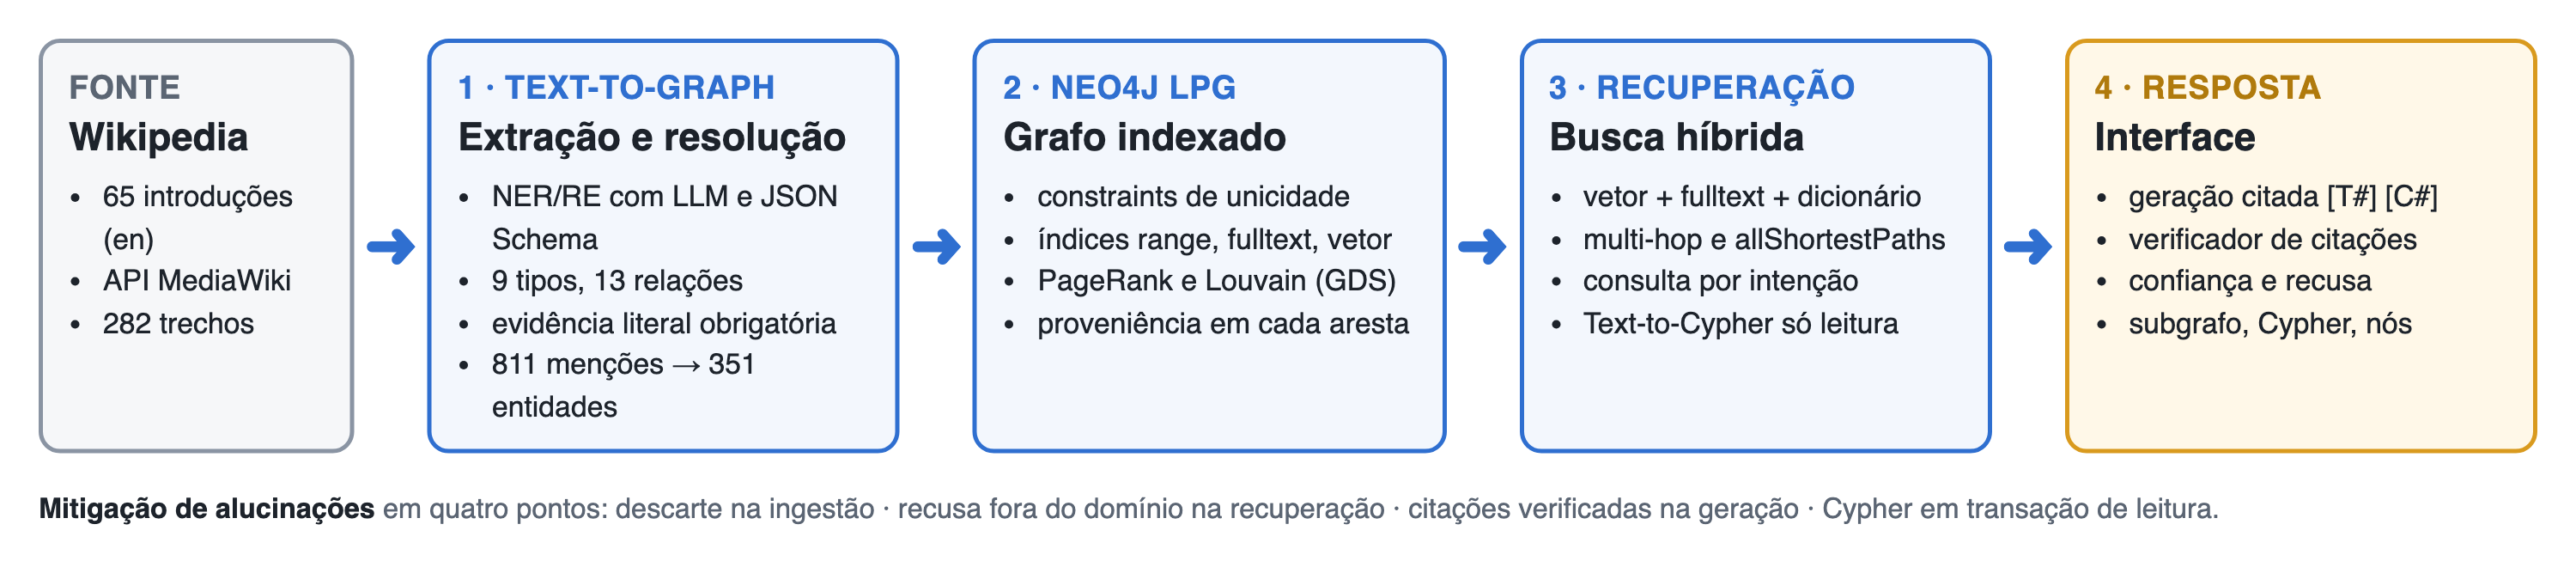
\includegraphics[width=\linewidth]{img/arquitetura.png}
\caption{Visão geral da arquitetura: as quatro etapas e os pontos de mitigação de alucinações.}
\end{figure}
\subsection{Corpus}
O corpus reúne a introdução de 65 artigos da Wikipedia em inglês, coletados pela API MediaWiki (\texttt{prop=extracts}, \texttt{exintro}, \texttt{explaintext}, seguindo redirecionamentos). A lista cobre jogos como Dota 2, League of Legends, Counter-Strike 2, Fortnite, PUBG: Battlegrounds, Minecraft, Roblox, World of Warcraft, Genshin Impact e Mobile Legends, além de jogos de origem histórica (Warcraft III, Defense of the Ancients, Arma 2, Half-Life) e dois campeonatos (The International e o mundial de League of Legends). Os textos são versionados em \texttt{data/raw/articles.json}, o que torna a carga reprodutível. Cada introdução é dividida em trechos de três frases, totalizando 282 trechos.

\subsection{Text-to-Graph: extração de entidades e relações}
A extração é feita por um LLM (Claude) com saída estruturada: o pedido inclui um JSON Schema derivado de modelos Pydantic, de modo que a resposta é sempre um objeto válido com \texttt{entities} e \texttt{relations}. O esquema fixa nove tipos de entidade (\texttt{Game}, \texttt{Company}, \texttt{Person}, \texttt{Genre}, \texttt{Platform}, \texttt{Engine}, \texttt{Franchise}, \texttt{Event}, \texttt{Concept}) e treze tipos de relação, entre eles \texttt{DEVELOPED\_BY}, \texttt{PUBLISHED\_BY}, \texttt{BASED\_ON}, \texttt{SEQUEL\_OF}, \texttt{CREATED\_BY}, \texttt{SUBSIDIARY\_OF}, \texttt{FEATURED\_IN} e \texttt{ORGANIZED\_BY}. O prompt pede nomes canônicos em inglês (por exemplo, ``Valve'' e não ``Valve Corporation'') e aliases explícitos.

Cada relação traz o campo \texttt{evidence}, a frase do texto que a sustenta. Um validador descarta toda relação cuja evidência não aparece literalmente no artigo, após normalização de espaços e caixa, e toda relação cujos extremos não estão entre as entidades extraídas. Essa é a primeira barreira contra alucinação: um fato só entra no grafo se puder ser apontado no texto. As 65 extrações somam 811 entidades e 797 relações; nenhuma relação foi rejeitada pelo validador de evidência e 1 foi descartada na carga porque, após a resolução de entidades, origem e destino viraram o mesmo nó. As extrações ficam versionadas em \texttt{data/extracted/}, e a carga do grafo não depende de chave de API.

\subsection{Resolução de entidades}
O mesmo jogo ou empresa aparece com nomes diferentes em artigos diferentes (``Valve'' e ``Valve Corporation'', ``Warcraft III'' e ``Warcraft III: Reign of Chaos'', ``MOBA'' e ``Multiplayer online battle arena''). A resolução usa união-busca (\emph{union-find}) em três passos:

\begin{enumerate}\item \textbf{Chave lexical.} Minúsculas, sem pontuação, sem plural simples e sem conteúdo entre parênteses, sempre dentro do mesmo tipo: a série \emph{Counter-Strike} e o jogo \emph{Counter-Strike} não se fundem.
\item \textbf{Aliases compatíveis.} Duas menções se fundem se o nome de uma é alias da outra e os nomes são compatíveis: mesma chave, sigla, trigramas parecidos, mesmo núcleo após remover sufixos corporativos (``Valve'' e ``Valve Corporation'') ou mesmo título-base antes do subtítulo (``Warcraft III'' e ``Warcraft III: Reign of Chaos''). Nomes com números diferentes nunca se fundem (\emph{Overwatch} e \emph{Overwatch 2}, \emph{PlayStation 4} e \emph{PlayStation 5}).
\item \textbf{Semântica.} Representantes do mesmo tipo e com os mesmos números se fundem se o cosseno entre embeddings é pelo menos 0,93 e a similaridade de trigramas é pelo menos 0,85.
\end{enumerate}
A trava lexical no passo 3 veio de um erro observado: só com embeddings, nomes curtos e diferentes do mesmo campo ficavam próximos e eram fundidos. Os testes unitários cobrem esses casos (por exemplo, \emph{Dota 2} e \emph{Dota Underlords}, \emph{Valve} e \emph{Valorant} não se fundem). O resultado foi de 811 menções para 351 entidades canônicas, das quais 93 aparecem em mais de um artigo e funcionam como pontes entre documentos.

\subsection{Modelagem no Neo4j}
O grafo segue o modelo LPG:

\begin{itemize}\item \texttt{(:Article \{doc\_id, title, text, url, embedding\})-[:DESCRIBES]->(:Entity)}, ligando cada artigo à entidade que ele descreve;
\item \texttt{(:Chunk \{id, text, embedding\})-[:PART\_OF]->(:Article)};
\item \texttt{(:Entity:Game|Company|...\{id, name, aliases, description, mentions, embedding, pagerank, community\})};
\item arestas tipadas entre entidades, cada uma com \texttt{evidence} e \texttt{doc\_id} (proveniência).
\end{itemize}
A Tabela 1 resume o grafo carregado. O esquema define restrições de unicidade em \texttt{Article.doc\_id}, \texttt{Entity.id} e \texttt{Chunk.id}, índices range (B-tree) em nome, tipo e PageRank das entidades e no título dos artigos, índices fulltext (Lucene) sobre nome, aliases e descrição das entidades e sobre título e texto dos artigos, e três índices vetoriais de 384 dimensões com similaridade de cosseno (entidades, trechos e artigos). Os embeddings vêm do modelo \texttt{intfloat/multilingual-e5-small}, executado localmente, o que permite perguntas em português sobre textos em inglês.

\begin{table}[ht]\centering\small
\caption{Composição do grafo carregado.}
\begin{tabular}{p{0.62\linewidth}r}\toprule
\textbf{Elemento} & \textbf{Quantidade} \\ \midrule
Artigos & 65 \\
Trechos & 282 \\
Entidades (Game 144, Company 75, Platform 25, Concept 25, Event 23, Person 18, Genre 18, Franchise 16, Engine 7) & 351 \\
Relações entre entidades (13 tipos) & 796 \\
Entidades presentes em mais de um artigo & 93 \\
Comunidades Louvain & 24 \\
\bottomrule\end{tabular}
\end{table}
Após a carga, o GDS projeta as entidades como grafo não direcionado e grava \texttt{pagerank} e \texttt{community} em cada nó. O PageRank é usado na recuperação de duas formas opostas: para ordenar a vizinhança multi-hop (nós centrais primeiro) e para preferir, entre caminhos mínimos de mesmo tamanho, os que passam por nós pouco centrais, já que um caminho por ``Windows'' ou ``Free-to-play'' quase nunca explica nada. O Louvain encontrou 24 comunidades com modularidade 0,53, algumas delas reconhecíveis (Valve e Counter-Strike; Blizzard, Warcraft e DotA; MOBAs mobile asiáticos; battle royale; Half-Life e seus mods), enquanto outras se formam em torno de plataformas compartilhadas, como consoles e celulares.

\subsection{Recuperação híbrida}
Dada uma pergunta, a recuperação executa os passos abaixo. Todas as consultas Cypher executadas são registradas com parâmetros e exibidas na interface.

\begin{enumerate}\item \textbf{Ligação de entidades por três canais.} (a) busca vetorial no índice de entidades com a pergunta prefixada por \texttt{query:}; (b) busca fulltext com a pergunta convertida em consulta Lucene, sem palavras vazias e com caracteres especiais escapados; (c) dicionário de nomes e aliases, mais um glossário português-inglês do domínio (``gratuito'' $\rightarrow$ \emph{Free-to-play}, ``tiro tático'' $\rightarrow$ \emph{Tactical shooter}). As listas são fundidas por RRF \cite{cormack2009rrf}, com bônus para correspondência exata.
\item \textbf{Âncoras.} São âncoras as entidades citadas literalmente na pergunta e as confirmadas ao mesmo tempo pelos canais vetorial e fulltext. A busca vetorial de trechos também ancora a entidade descrita pelo artigo do trecho mais próximo.
\item \textbf{Travessia multi-hop.} Caminhos de comprimento variável (\texttt{[*1..h]}, com $h = 2$ por padrão e até 3) a partir das sementes, restritos a nós \texttt{Entity}.
\item \textbf{Caminhos mínimos.} \texttt{allShortestPaths} entre cada par de âncoras, até 3 por par, ordenados pela menor soma de PageRank.
\item \textbf{Consulta dirigida pela intenção.} Expressões da pergunta (``quem criou'', ``desenvolveu'', ``subsidiária'', ``campeonato'') são mapeadas em tipos de relação. Uma consulta busca essas relações a partir das âncoras e de seus vizinhos diretos. Esse passo foi incluído porque o corte da travessia por PageRank descartava fatos sobre nós específicos, como pessoas e estúdios pequenos (Listagem 1).
\item \textbf{Reordenação.} Cada tripla recebe a similaridade de cosseno entre a pergunta e o texto ``sujeito relação objeto. evidência'', mais bônus por estar em caminho mínimo, por ter o tipo pedido e por tocar uma âncora. As 30 melhores formam o contexto, junto com os quatro trechos mais próximos.
\end{enumerate}
\begin{lstlisting}[caption={Consulta dirigida pela intenção (simplificada).}]
MATCH (s:Entity) WHERE elementId(s) IN $anchors
MATCH (s)-[*0..1]-(m:Entity)-[r]-(:Entity) WHERE type(r) IN $rels
WITH DISTINCT r LIMIT 60
RETURN type(r) AS rel, r.evidence AS evidence, r.doc_id AS doc_id,
       startNode(r).name AS src, endNode(r).name AS dst
\end{lstlisting}
\textbf{Text-to-Cypher.} Quando há chave de API, o LLM recebe a descrição do esquema e gera uma consulta Cypher para a pergunta. A consulta passa por um filtro que remove literais e comentários e rejeita cláusulas de escrita e procedimentos perigosos (\texttt{CREATE}, \texttt{MERGE}, \texttt{DELETE}, \texttt{SET}, \texttt{LOAD CSV}, \texttt{apoc.create}, \texttt{dbms.*}, \texttt{gds.*.write}), recebe \texttt{LIMIT} se não tiver e roda em transação de leitura do driver. Mesmo que o filtro falhe, o banco rejeita a escrita. O resultado entra no contexto como evidência adicional.

\subsection{Geração e mitigação de alucinações}
O contexto entregue ao LLM numera as triplas (\texttt{[T1]}, \texttt{[T2]}...) com sua evidência e seu artigo de origem, e os trechos (\texttt{[C1]}...). O prompt de sistema exige que toda afirmação termine com citação, que caminhos multi-hop sejam explicados salto a salto e que, sem contexto suficiente, a resposta seja exatamente ``Não encontrei essa informação no grafo.''. Depois da geração, um verificador remove citações para identificadores inexistentes e conta frases longas sem nenhuma citação.

O nível de confiança combina três componentes: ligação (força da correspondência da pergunta com o grafo, 40\%), estrutura (caminho entre âncoras ou triplas suficientes, 30\%) e fundamentação (fração de frases com citação válida, 30\%). Uma pergunta é considerada fora do domínio quando nenhuma entidade é citada literalmente e a maior similaridade vetorial fica abaixo de um limiar. Nesse caso o sistema recusa antes de gerar. O limiar foi calibrado em 0,924 a partir das distribuições observadas: perguntas fora do domínio ficaram entre 0,893 e 0,922; paráfrases do domínio sem nomes próprios ficaram entre 0,920 e 0,933. Escolhemos o lado conservador: uma das quatro paráfrases testadas passa a ser recusada.

Sem chave de API, o sistema roda em modo extrativo: a resposta é montada das triplas mais relevantes, agrupadas por sujeito, priorizando a relação pedida e as entidades citadas, e cada frase cita a tripla de origem. Esse modo garante que a demonstração e a avaliação não dependam de serviço externo.

\subsection{Interface}
A interface em Streamlit (Figura 2) recebe a pergunta e permite escolher o modo de recuperação (GraphRAG ou só vetorial), o número de saltos e o uso do LLM. Ela mostra: a resposta com citações clicáveis; o subgrafo interativo, com cores por tipo, caminhos mínimos destacados e a opção de destacar uma tripla citada; o nível de confiança e seus três componentes; as entidades ligadas e por qual canal; e abas com as triplas (com evidência e link para o artigo), as consultas Cypher executadas com parâmetros (Figura 3), os nós consultados, os trechos, os tempos de cada etapa e a avaliação.

\begin{figure}[ht]\centering
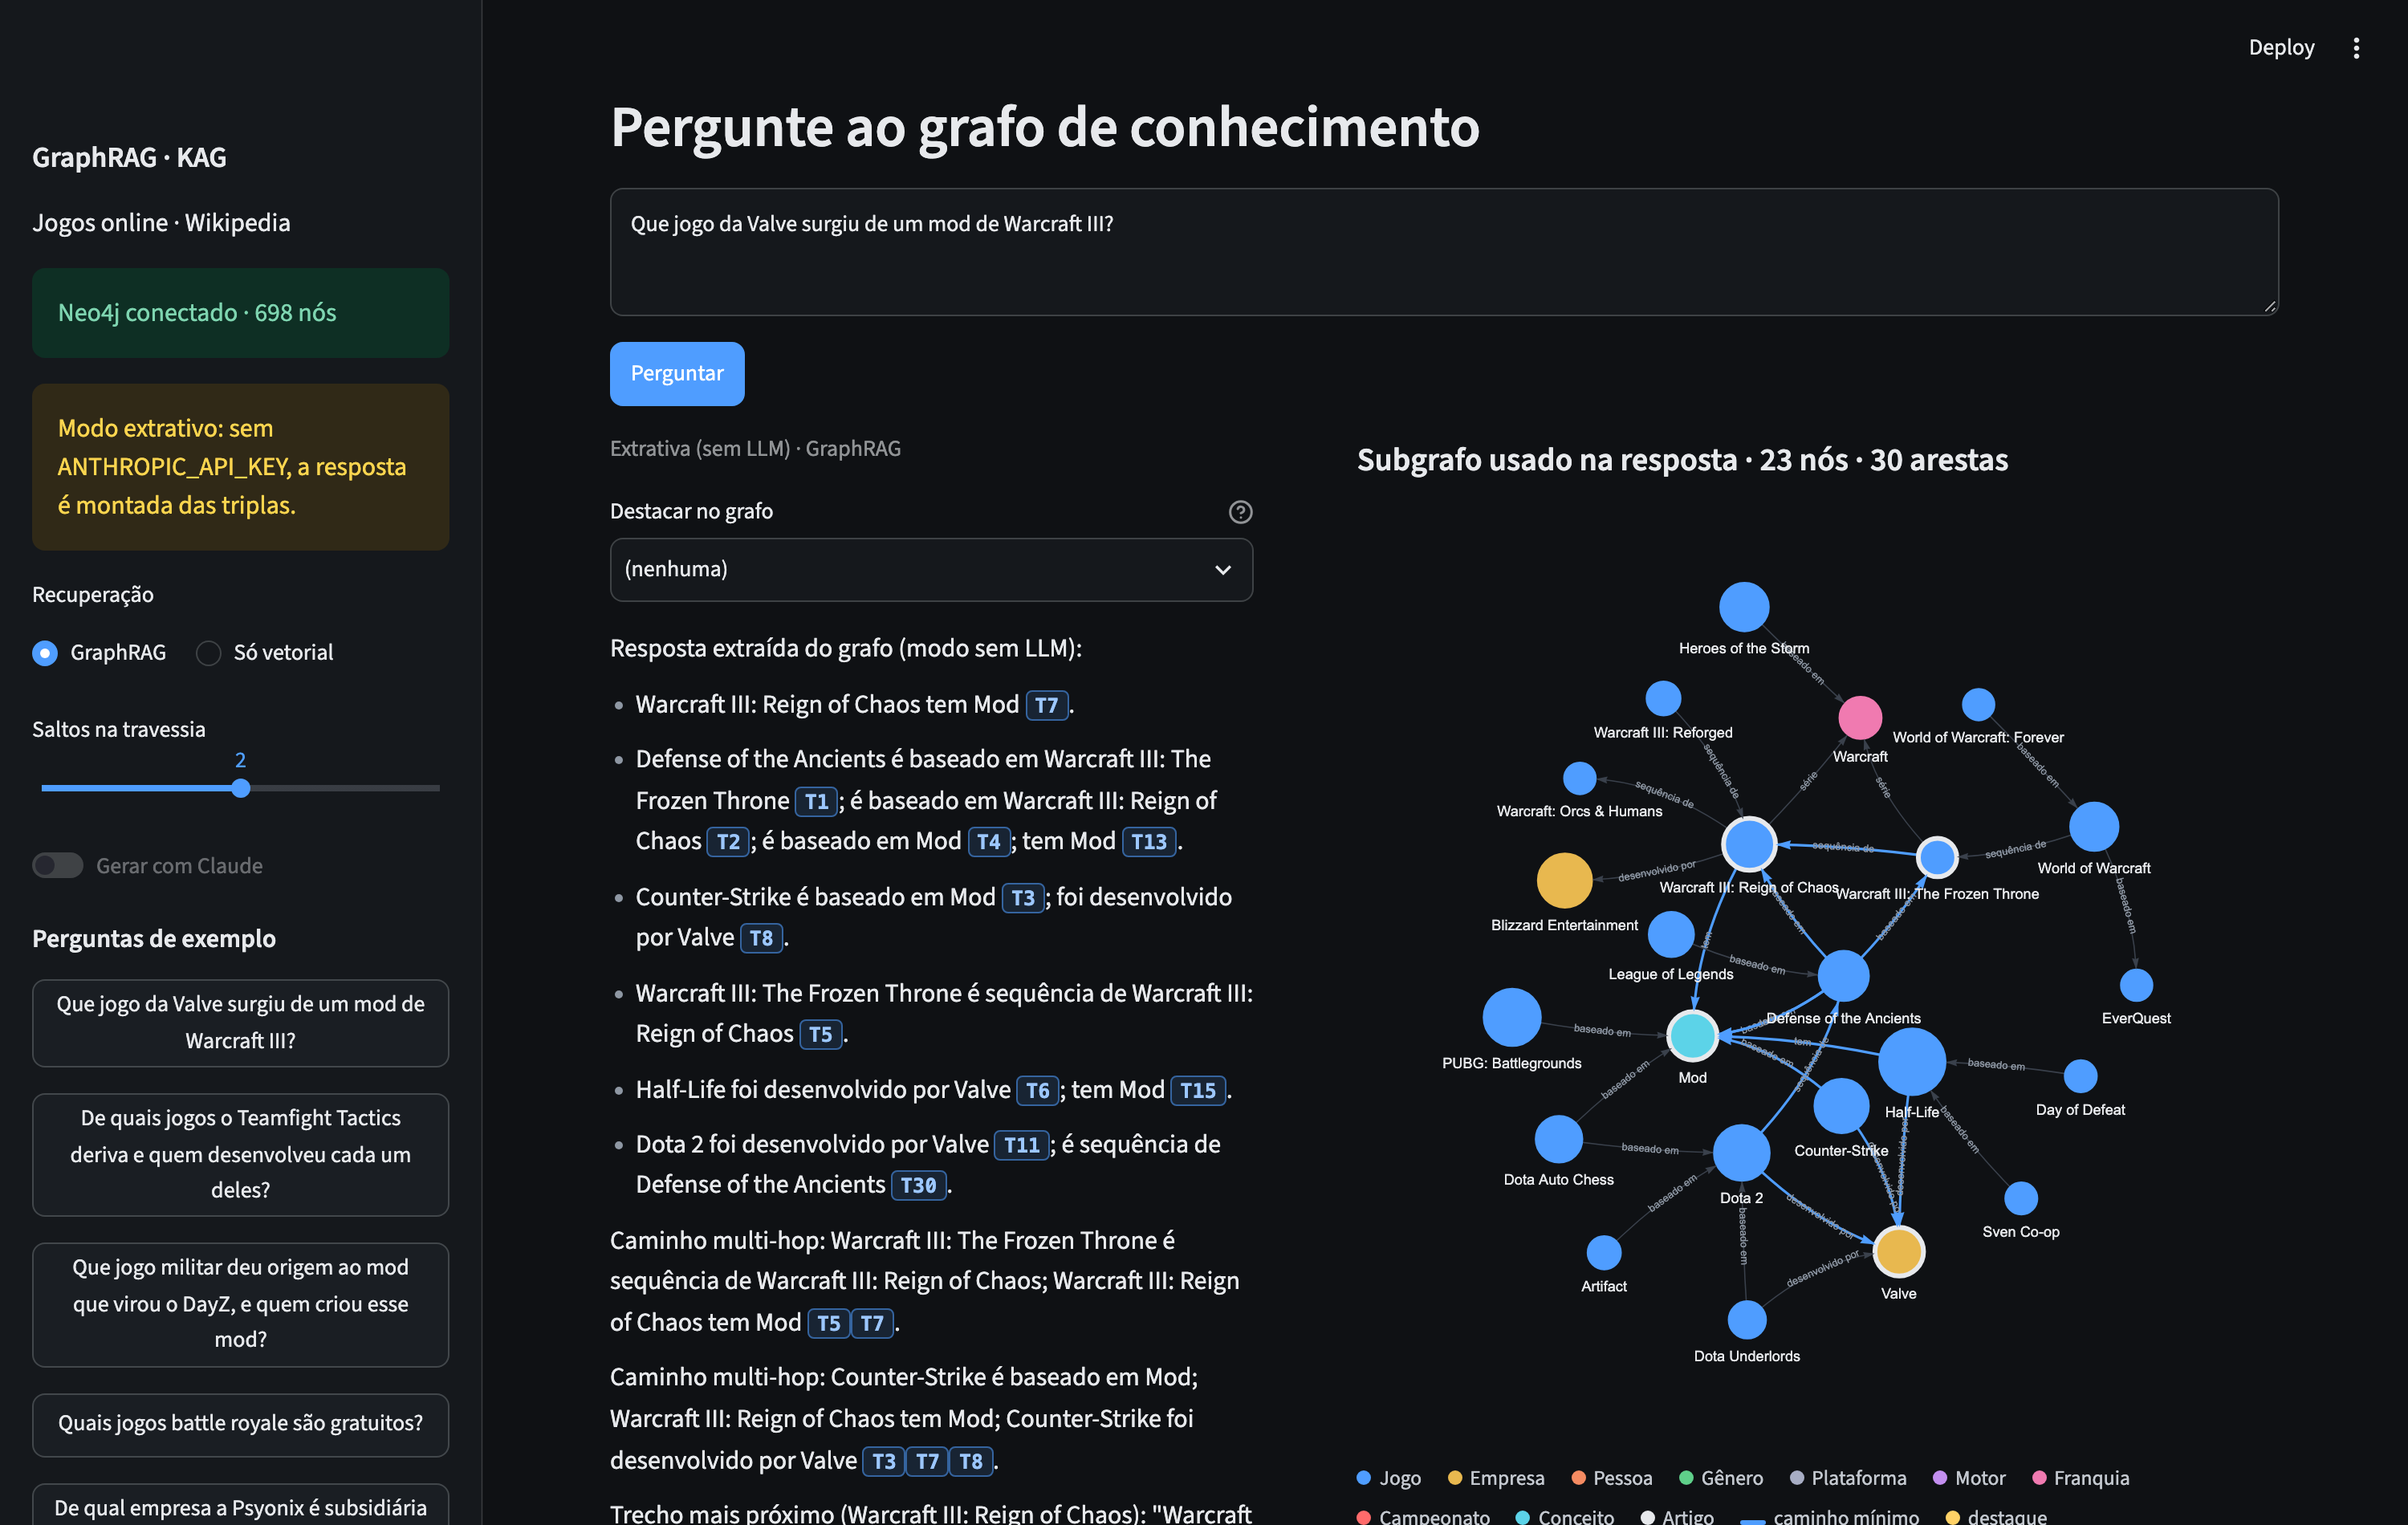
\includegraphics[width=\linewidth]{img/ui-multihop.png}
\caption{Interface respondendo uma pergunta de vários saltos: resposta citada à esquerda e subgrafo usado à direita.}
\end{figure}
\begin{figure}[ht]\centering
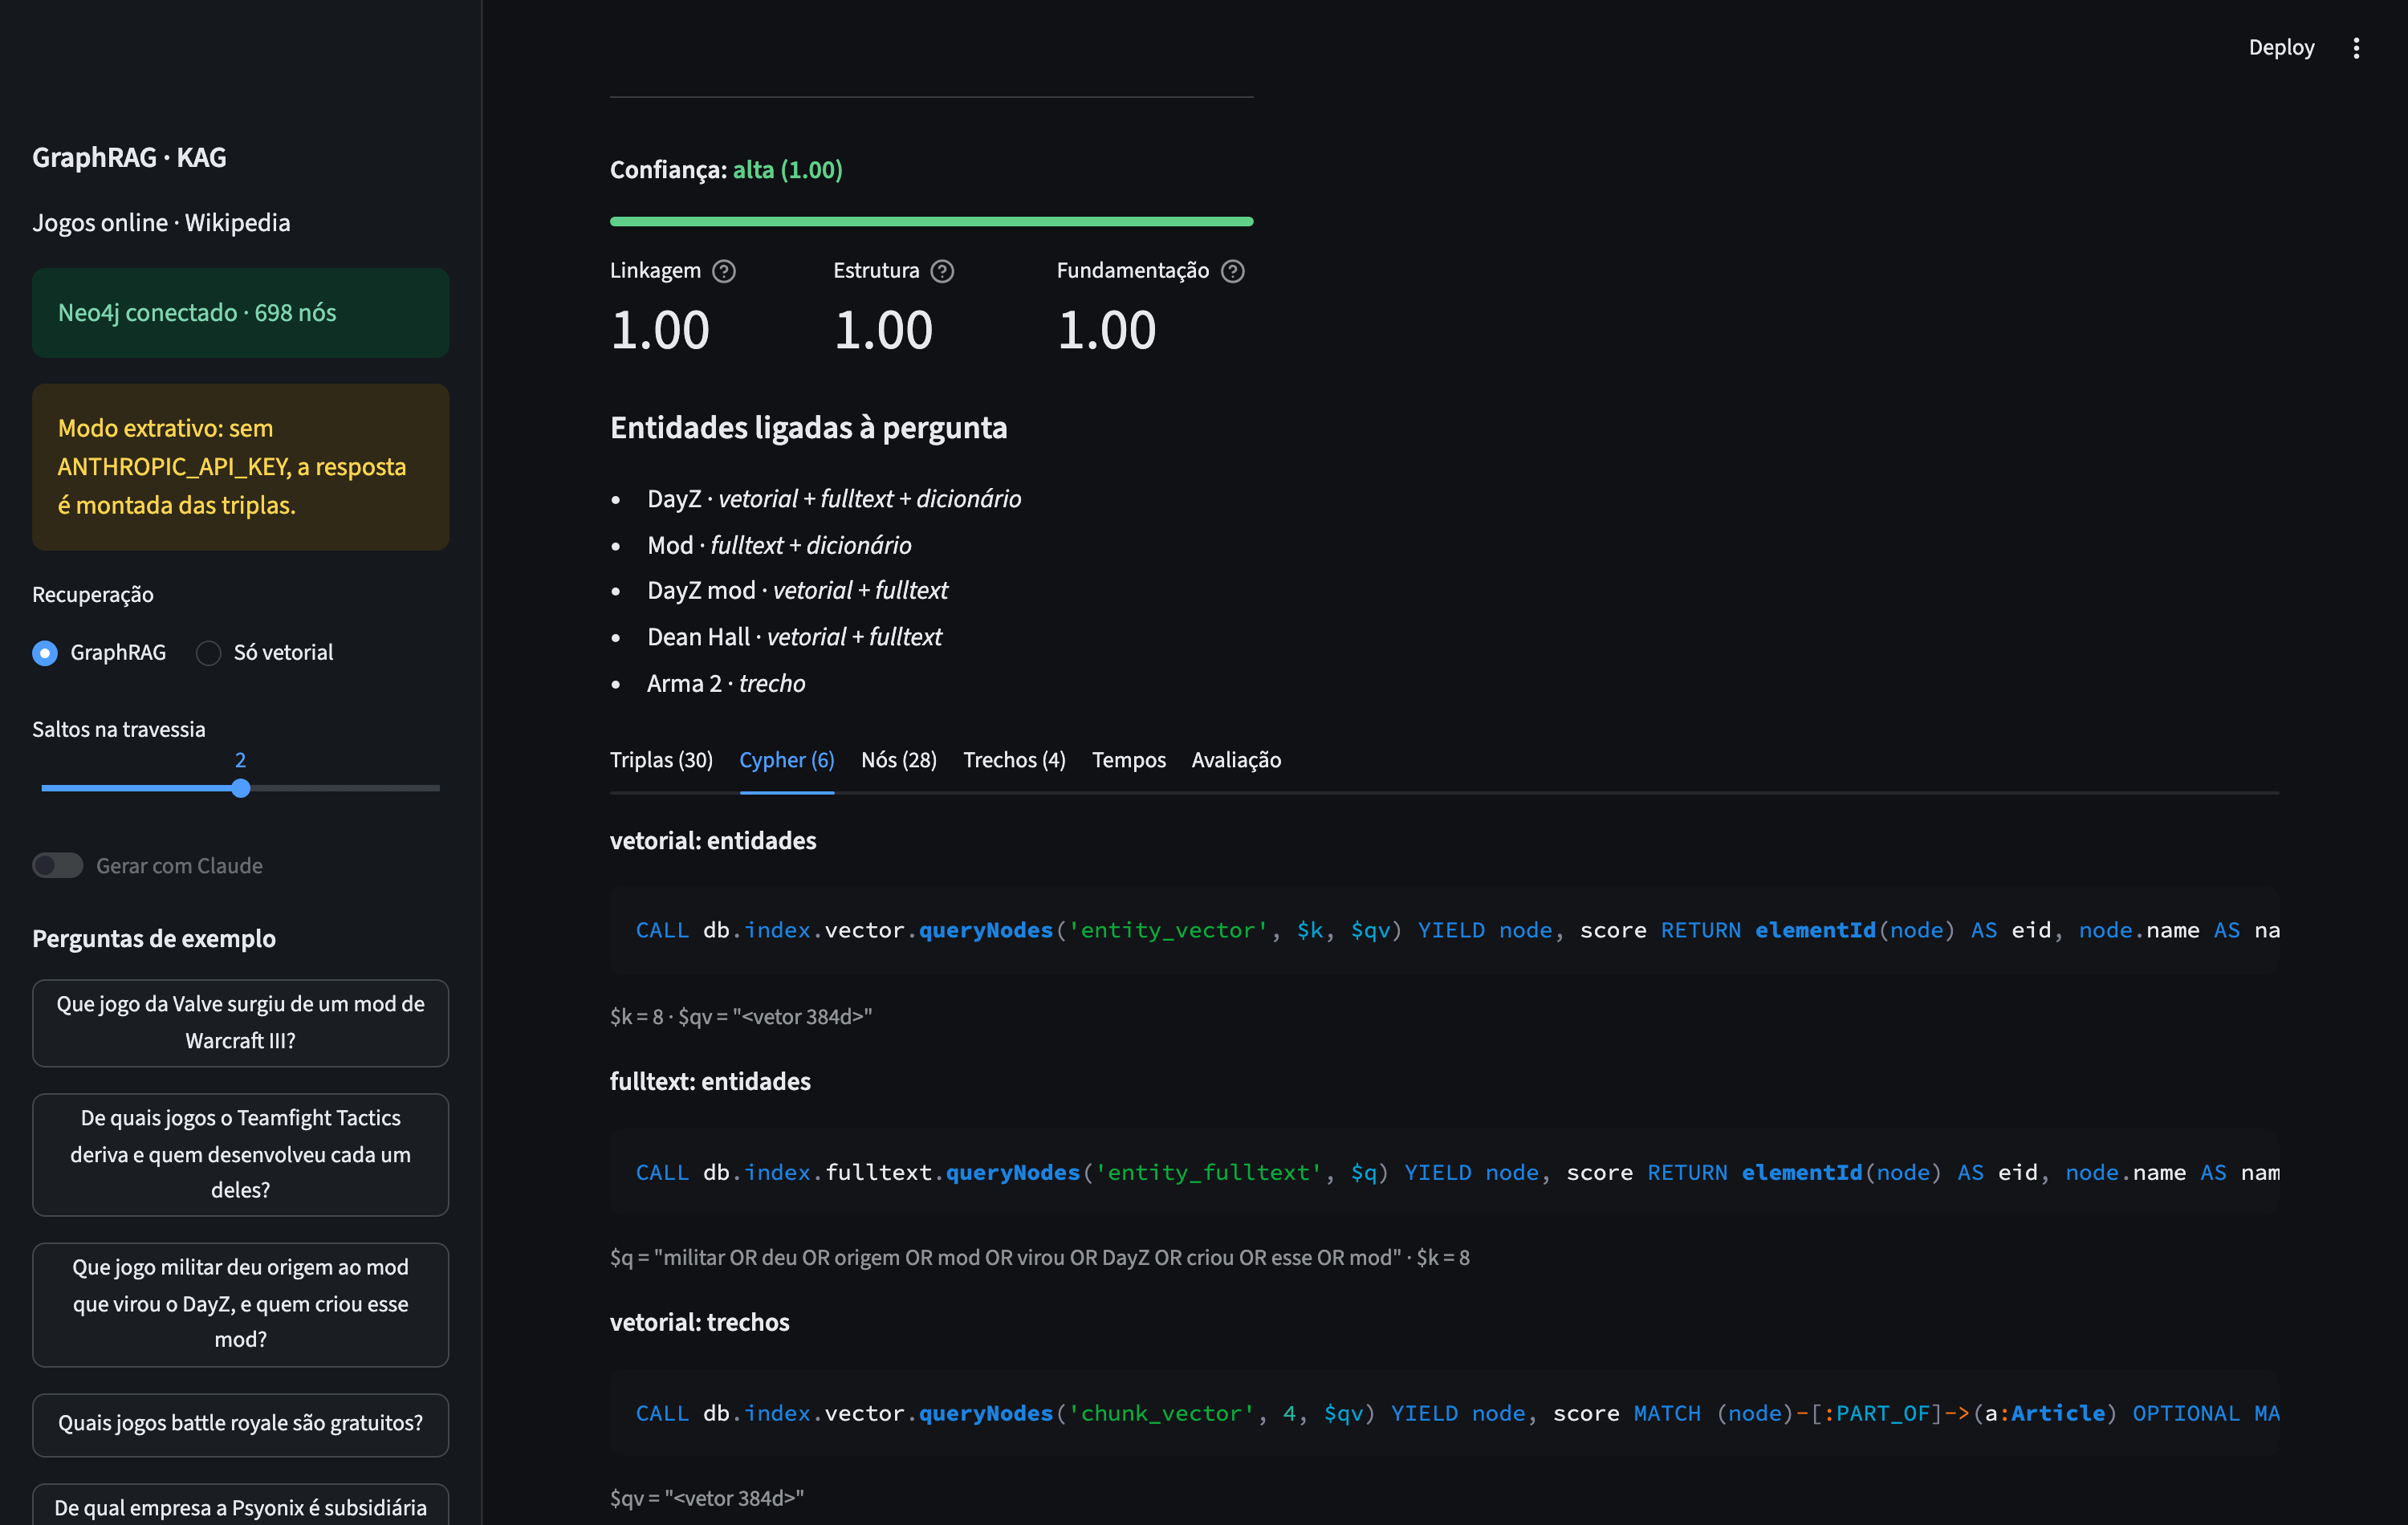
\includegraphics[width=\linewidth]{img/ui-cypher.png}
\caption{Aba de proveniência com as consultas Cypher executadas e as entidades ligadas a cada canal.}
\end{figure}
\section{Avaliação}
\subsection{Protocolo}
Comparamos o contexto produzido pelo GraphRAG com o de um baseline de RAG vetorial puro, que recupera os oito trechos mais próximos no mesmo índice vetorial e com o mesmo modelo de embeddings. Medimos o contexto, e não a resposta, porque ele determina o que qualquer gerador pode afirmar com respaldo; assim a avaliação também roda sem chave de API.

O conjunto tem 26 perguntas em português: 12 de um salto, 9 de dois ou mais saltos e 5 fora do domínio (receitas, geografia, futebol, biologia, dieta). Cada pergunta do domínio tem um gabarito, isto é, a lista de itens que precisam aparecer no contexto, com sinônimos aceitos. Os gabaritos foram conferidos contra as triplas e os textos. As métricas são: recall no contexto (fração dos itens do gabarito presentes), suporte completo (todos os itens presentes), tamanho do contexto, latência de recuperação e taxa de abstenção correta (fora do domínio) e indevida (no domínio).

\subsection{Resultados}
\begin{table}[ht]\centering\small
\caption{GraphRAG contra RAG vetorial (26 perguntas; latência medida em notebook, Neo4j local).}
\begin{tabular}{lrr}\toprule
\textbf{Métrica} & \textbf{GraphRAG} & \textbf{RAG vetorial} \\ \midrule
Recall no contexto (21 perguntas) & 1,000 & 0,853 \\
Suporte completo & 100\% & 71,4\% \\
Recall, 1 salto (12) & 1,000 & 0,917 \\
Recall, 2+ saltos (9) & 1,000 & 0,769 \\
Tamanho médio do contexto (caracteres) & 7.159 & 2.352 \\
Latência mediana de recuperação (ms) & 320 & 14 \\
Abstenção correta fora do domínio (5) & 100\% & 0\% \\
Abstenção indevida no domínio & 0\% & 0\% \\
\bottomrule\end{tabular}
\end{table}
O ganho se concentra nas perguntas de vários saltos. Em ``O Counter-Strike é um mod de qual jogo, e quem são os criadores do mod?'', o baseline encontra o \emph{Half-Life}, mas não os criadores, que estão em outro artigo; o grafo liga \emph{Counter-Strike} $\rightarrow$ \texttt{BASED\_ON} $\rightarrow$ \emph{Half-Life} e \emph{Counter-Strike} $\rightarrow$ \texttt{CREATED\_BY} $\rightarrow$ \emph{Minh Le}, \emph{Jess Cliffe}. Em ``Que jogo da Valve surgiu de um mod de Warcraft III?'', o caminho \emph{Dota 2} $\rightarrow$ \texttt{SEQUEL\_OF} $\rightarrow$ \emph{Defense of the Ancients} $\rightarrow$ \texttt{BASED\_ON} $\rightarrow$ \emph{Warcraft III} cruza três artigos. Nas perguntas de um salto, o baseline também vai bem (0,917), já que as introduções da Wikipedia são curtas e concentradas; sua falha típica é um fato citado de passagem em outro artigo, como o criador do PUBG.

Fora do domínio, o grafo recusou as cinco perguntas e o baseline respondeu todas com os trechos menos distantes, que não têm relação com a pergunta. O custo do GraphRAG é um contexto cerca de três vezes maior e latência de recuperação de centenas de milissegundos, ainda pequena diante do tempo de geração de um LLM.

\subsection{Testes operacionais}
O repositório inclui 28 testes automatizados. Os 19 unitários cobrem resolução de entidades, trava de somente leitura do Cypher, verificador de citações, validação de evidência, montagem do grafo e utilitários. Os 9 de integração rodam contra o Neo4j carregado e verificam: existência de restrições e dos três tipos de índice; evidência e \texttt{doc\_id} em toda relação; propriedades do GDS em todo nó; rejeição de escrita na transação de leitura; recuperação multi-hop cruzando mais de um artigo; recusa fora do domínio; e proveniência completa na API.

\section{Limitações e ameaças à validade}
\begin{itemize}\item \textbf{Conjunto de avaliação pequeno e não independente.} As perguntas foram escritas pela equipe a partir de fatos conhecidos do grafo, e dois ajustes (a consulta dirigida pela intenção e o limiar de recusa) foram feitos depois de observar falhas nesse mesmo conjunto. O resultado de 100\% deve ser lido como evidência de que o mecanismo funciona, não como estimativa de desempenho em perguntas novas. Um conjunto separado, escrito por pessoas fora da equipe, é o próximo passo.
\item \textbf{Medida no contexto.} Ter o fato no contexto é condição necessária, não suficiente, para uma resposta correta; a avaliação da resposta gerada exige a chave de API (\texttt{run\_eval --llm}).
\item \textbf{Extração.} A extração versionada foi gerada com Claude seguindo o mesmo prompt e esquema do código, e validada automaticamente, mas não foi revisada manualmente por completo. Escolhas de tipo de relação (por exemplo, remake como \texttt{SEQUEL\_OF}) afetam quais caminhos existem.
\item \textbf{Cobertura.} Só as introduções dos artigos foram usadas; fatos conhecidos, como a Riot Games pertencer à Tencent, não aparecem nelas e, corretamente, não estão no grafo.
\item \textbf{Limiar de recusa.} A calibração usa poucas perguntas e o modelo de embeddings dá similaridades altas para quase tudo; a faixa entre domínio e fora do domínio é estreita.
\end{itemize}
\section{Conclusão}
Construímos um sistema GraphRAG/KAG completo sobre jogos online, da coleta na Wikipedia à interface com proveniência. A combinação de extração com evidência literal, resolução de entidades com travas lexicais, modelagem LPG com índices e algoritmos de grafo e recuperação híbrida com caminhos mínimos permitiu juntar fatos de artigos diferentes que a busca vetorial não reúne, e deu ao sistema um critério objetivo para recusar perguntas fora da base. Como trabalhos futuros, apontamos: avaliar com perguntas independentes e com respostas geradas; usar o texto completo dos artigos; resumir comunidades Louvain para perguntas globais, como no GraphRAG; e atualizar o grafo de forma incremental.

O código, os dados e as instruções de execução estão no repositório do projeto.

\IfFileExists{sbc.bst}{\bibliographystyle{sbc}}{\bibliographystyle{apalike}}
\bibliography{referencias}
\end{document}
